\documentclass[letterpaper,12pt]{article}

%\usepackage{ucs}
%\usepackage[utf8x]{inputenc}
\usepackage{amsmath}
\usepackage{amsfonts}
\usepackage{amssymb}
\usepackage{graphicx}
%\usepackage[canadian]{babel}
\usepackage[margin=1in]{geometry}
\usepackage{multicol}
\newcommand{\R}{\mathbb{R}}
\renewcommand{\i}{\mathbf{i}}
\renewcommand{\j}{\mathbf{j}}
\renewcommand{\k}{\mathbf{k}}
\newcommand{\pd}[2]{\dfrac{\partial #1}{\partial #2}}
\newcommand{\di}{\displaystyle}
\renewcommand{\phi}{\varphi}

\title{Solutions to Quiz 12 Practice\\Math 2580\\Spring 2016}
\author{Sean Fitzpatrick}
\date{March 1st, 2016}

\begin{document}
 \maketitle

\begin{enumerate}
 \item For the following double integral, sketch the region of integration, change the order of integration, and evaluate:
\[
 \int_1^4\int_1^{\sqrt{x}}(x^2+y^2)\,dy\,dx.
\]
Our region of integration is bounded above by $y=\sqrt{x}$ and below by $y=1$, for $1\leq x\leq 4$, which gives us the following Type 1 region:
\begin{center}
 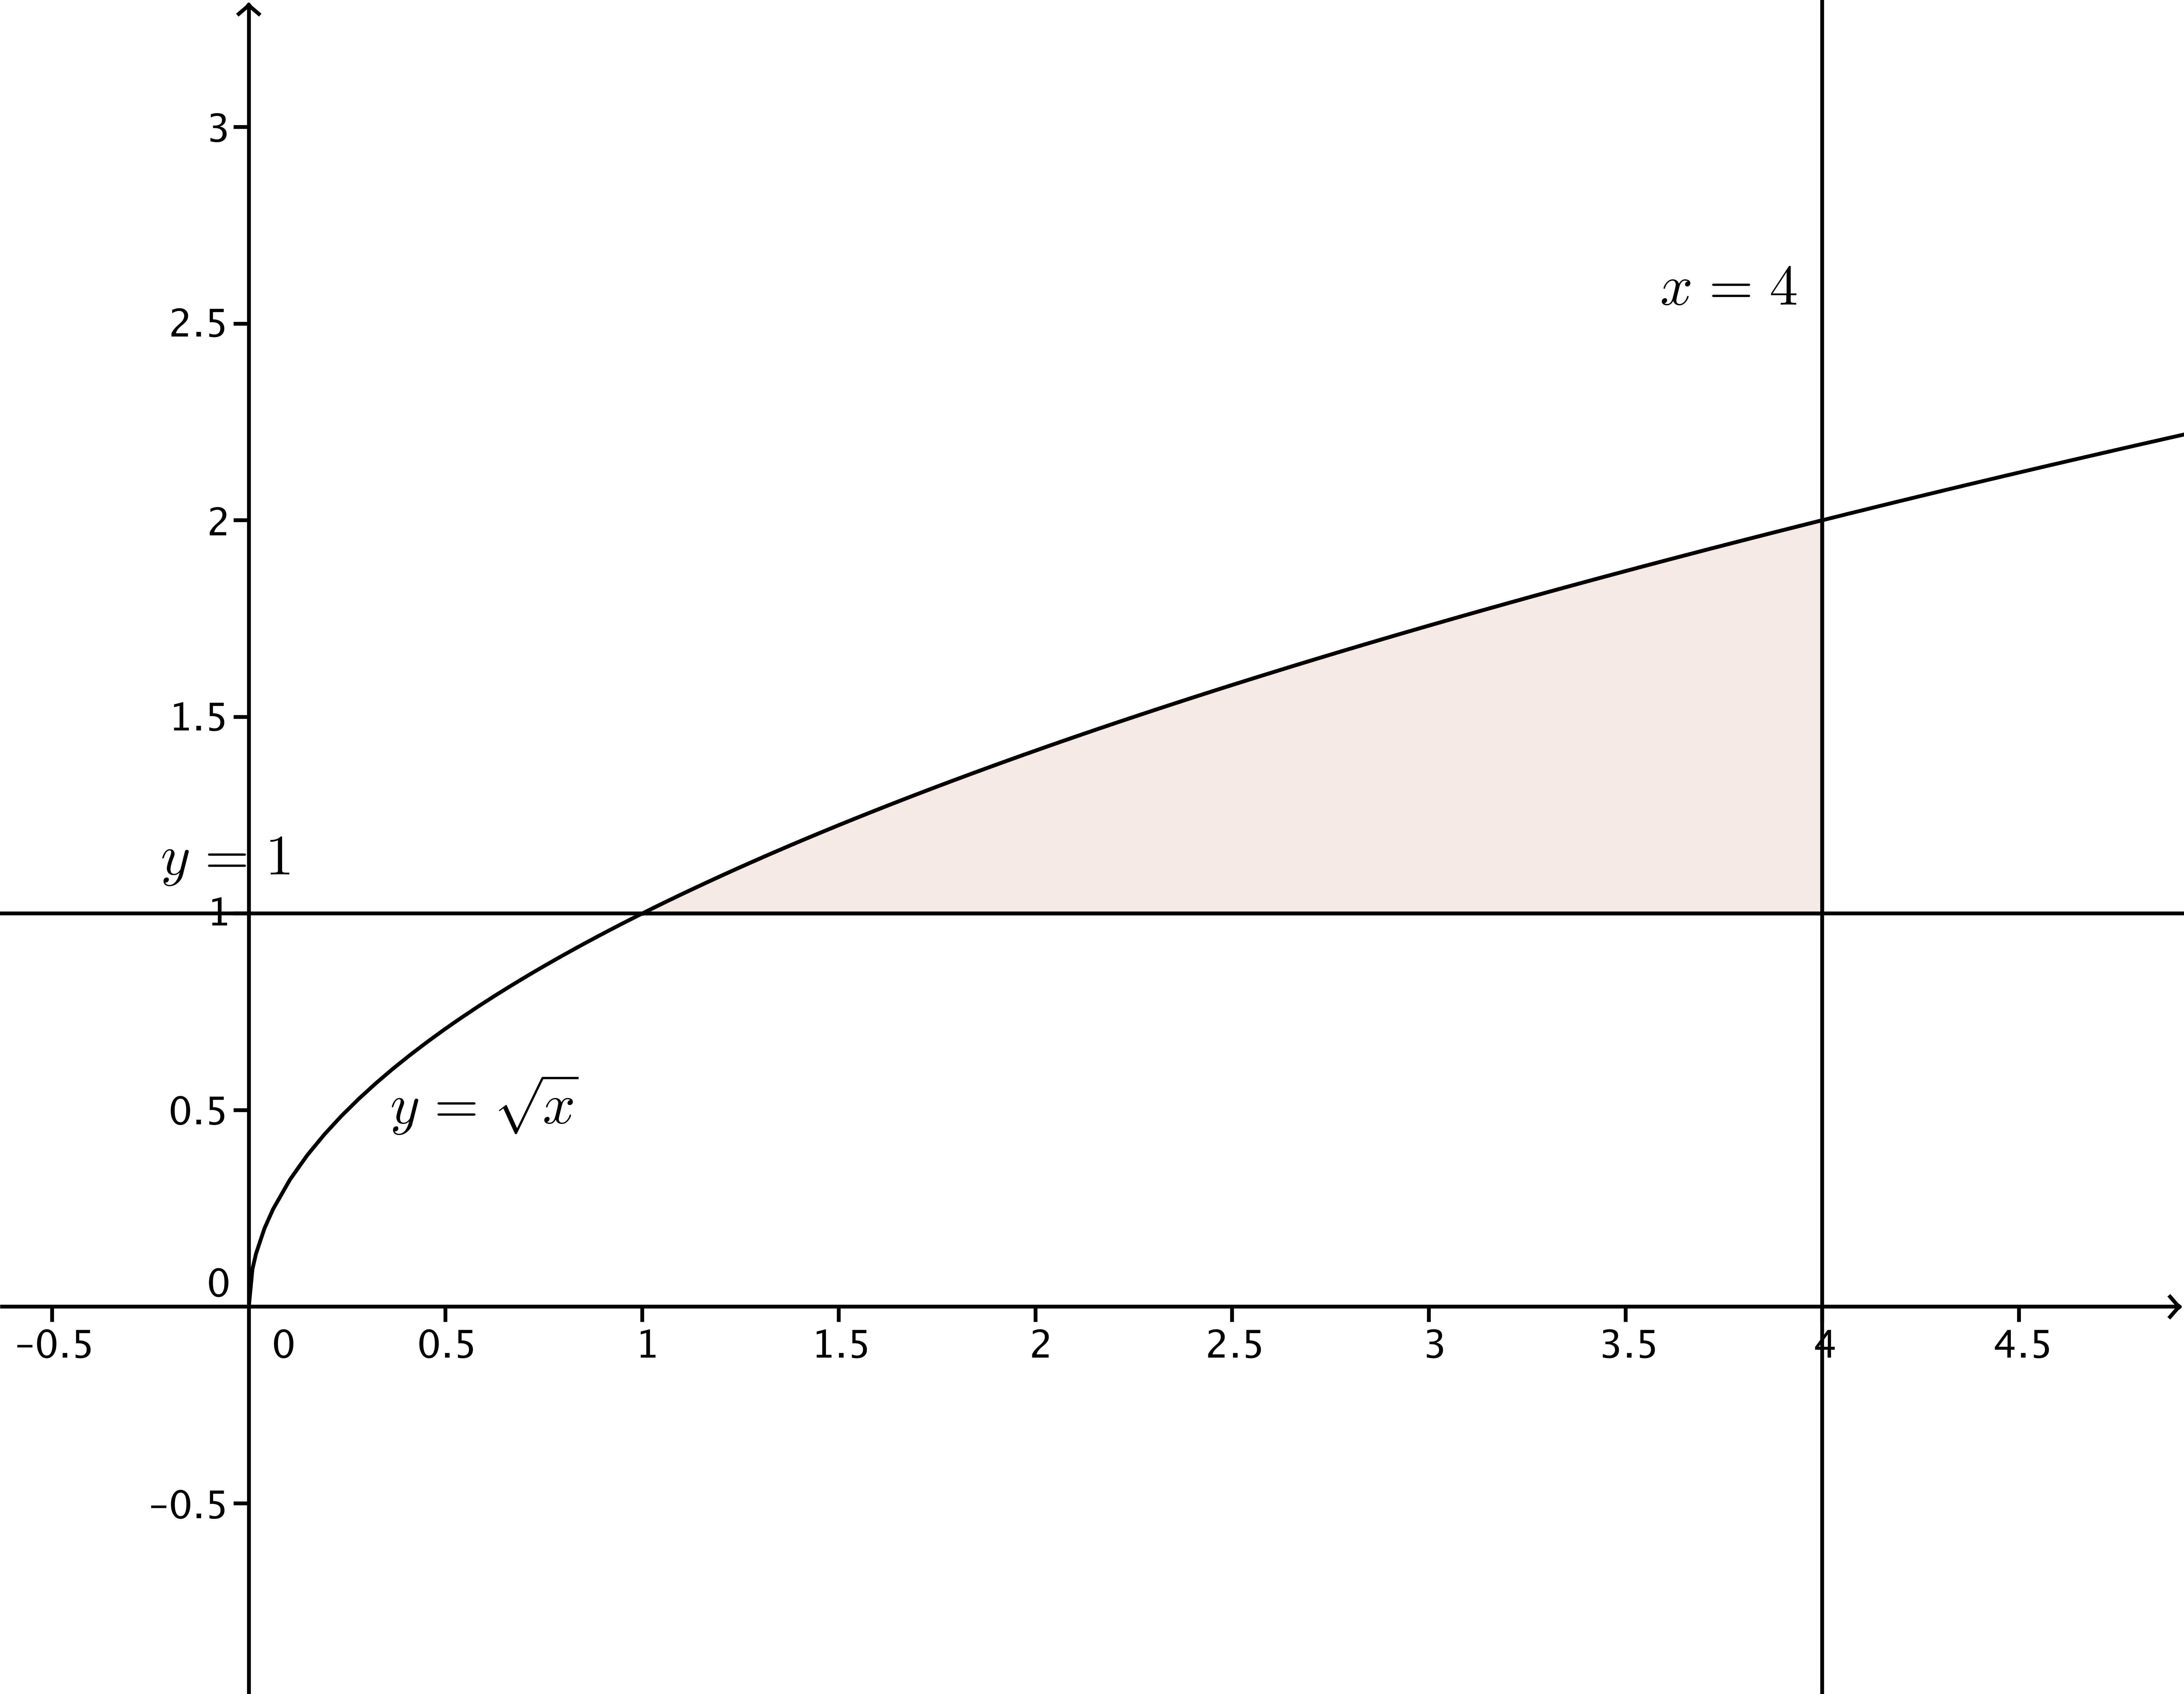
\includegraphics[width=0.5\textwidth]{Q12-1.png}
\end{center}
Reversing the order, we have the Type 2 region $y^2\leq x\leq 4$, for $1\leq y\leq 2$. Thus, we have
\begin{align*}
 \int_1^4\int_1^{\sqrt{x}} (x^2+y^2)\,dy\,dx & = \int_1^2\int_{y^2}^4(x^2+y^2)\,dx\,dy\\
& = \int_1^2\left(\left. \frac{1}{3}x^3+xy^2\right|_{x=y^2}^{x=4}\right)\,dy\\
& = \int_1^2\left(\frac{64}{3}-\frac{y^6}{3}+4y^2-y^4\right)\,dy\\
& = \left. \frac{64y}{3}-\frac{y^7}{21}+\frac{4y^3}{3}-\frac{y^5}{5}\right|_1^2\\
& = \frac{64}{3}(2-1)-\frac{1}{21}(2^7-1)+\frac{4}{3}(2^3-1)-\frac{1}{5}(2^5-1).
\end{align*}


 \item Evaluate the integral $\di \iiint_B x^2\,dV$, where $B=[0,1]\times [-1,1]\times [0,1]$.

\bigskip

We have
\[
 \iiint_B x^2\,dV = \int_0^1\int_{-1}^1\int_0^1 x^2\,dx\,dy\,dz = \int_0^1\int_{-1}^1 \frac{1}{3}\,dy\,dz = \int_0^1 \frac{2}{3}\,dz = \frac{2}{3}.
\]

 \item Write the integral $\di \iiint_W f(x,y,z)\,dV$, where $W$ is the region between the cone $z=\sqrt{x^2+y^2}$ and the paraboloid $z=x^2+y^2$, as an interated integral. (Start by describing $W$ using inequalities of the form $g_1(x,y)\leq z\leq g_2(x,y)$, where $(x,y)\in D$, and then describe $D$ as either a Type 1 or Type 2 region.)

\bigskip

The cone and parabola intersect when $\sqrt{x^2+y^2} = x^2+y^2$. Letting $r=\sqrt{x^2+y^2}$, this requires $r=r^2$, so $r=0$ or $r=1$. (Notice that the region of integration can be obtained by taking the area above the parabola $z=y^2$ and below the line $z=y$, and revolving about the $z$-axis.) So the two surfaces intersect at the origin, and again along the circle $x^2+y^2=1$ in the plane $z=1$.

We can thus describe our region via the inequalities $x^2+y^2\leq z\leq \sqrt{x^2+y^2}$, where $x^2+y^2\leq 1$. We can describe the disc $x^2+y^2\leq 1$ as the Type 1 region $-1\leq x\leq 1$, $-\sqrt{1-x^2}\leq y\leq \sqrt{1-x^2}$. Thus,
\[
 \iiint_W f(x,y,z)\,dV = \int_{-1}^1\int_{-\sqrt{1-x^2}}^{\sqrt{1-x^2}}\int_{x^2+y^2}^{\sqrt{x^2+y^2}}f(x,y,z)\,dz\,dy\,dx.
\]


 \item Evaluate the integral $\di \iiint_W z\,dV$, where $W$ is the region bounded by the cylinder $x^2+y^2=4$ and the planes $z=0$ and $z=1$.

\bigskip

Here, we have $0\leq z\leq 1$, where $x^2+y^2\leq 4$. Carrying out the integral over $z$, we have
\[
 \iiint_W z\,dV = \iint_D(\int_0^1 z\,dz)\,dA = \iint_D \frac{1}{2}\,dA = \frac{A(D)}{2},
\]
where $D$ is the disc $x^2+y^2\leq 4$. We know that this disc has area $A(D) = \pi(2)^2 = 4\pi$, so the result of the integral must be $2\pi$.

 \item Describe the surfaces given in cylindrical coordinates by (i) $r=3$, (ii) $\theta = \pi/4$, and (iii), $z=2$.

\bigskip

(i) This is the cylinder $x^2+y^2=9$.

(ii) This is the portion of the plane $x=y$ for which $x,y\geq 0$. (It is a vertical plane obtained by extending horizontally from the $z$-axis along the line $x=y$ for each $z$-value.

(iii) This is just the horizontal plane $z=2$, as usual.

 \item Express the surface $z=x^2+y^2$ in spherical coordinates.

\bigskip

In spherical coordinates we have $x=\rho\cos\theta\sin\phi$ and $y=\rho\sin\theta\sin\phi$, so
\[
 x^2+y^2 = \rho^2\cos^2\theta\sin^2\phi+\rho^2\sin^2\theta\sin^2\phi = \rho^2\sin^2\phi,
\]
and $z=\rho\cos\phi$. Equating the two gives $\rho\cos\phi = \rho^2\sin^2\phi$, which we can simplify to $\rho = \cot\phi\csc\phi$. (Note that this last equation still has $\rho=0$ as a solution, so we haven't lost the solution $\rho=0$ by cancelling $\rho$ from both sides.)
 \end{enumerate}

\end{document}
 
